
\section{Experiments}

\noindent\textbf{Revision status.} The results in this section are retained from the earlier RLAR implementation. They have not been rerun with the construction, validation, and group-scoring protocol in Section~\ref{sec:method}. The revised primary evaluation concerns objectively verifiable mathematics and code tasks; historical translation/dialogue results are not evidence for the new validation protocol.

% We evaluate \method{} in two stages. First, we validate the core reward routing and selection mechanism on \textsc{RewardBench-v2} to confirm the inherent correctness of the agentic reward design (\S\ref{sec:eval_routing}). Then, we deploy \method{} in full RL post-training across four diverse task domains to assess its end-to-end effectiveness.


\subsection{Dataset and Evaluation}

We conduct RL training and evaluation across four representative task domains, each chosen to stress-test different aspects of the reward system. \textbf{Math Reasoning:} We use \textsc{GSM8k}~\citep{gsm8k} and \textsc{Hendrycks-MATH}~\citep{hendrycks2021measuringmathematicalproblemsolving} for mathematical reasoning. The goal is to reason toward the final numeric solution. \textbf{Coding:} We select the \textsc{LeetCode-Dataset}~\citep{leetcodedataset}, which requires the model to fill in LeetCode cloze-style function implementations. \textbf{Translation:} We sample from \textsc{FLORES-101}~\citep{flores101} to cover 20 translation pairs across five languages (CN, DE, EN, FR, JP). This task requires mastery across languages and is important for LLMs' accessibility to worldwide users, especially non-English speakers. \textbf{General Alignment:} \textsc{UltraChat}~\citep{ultrachat} is employed to train and evaluate multi-turn dialogue and instruction-following capabilities.


\noindent\textbf{Generalization Challenge.}\quad To assess the robustness of the trained policy, we include benchmarks such as \textsc{AIME-24/25} for math reasoning, \textsc{MBPP}~\citep{mbpp} for Python synthesis, and \textsc{WMT-24} for unseen translation contexts. 
These benchmarks evaluate whether the post-trained model can generalize rather than overfit to the specific heuristics of the training reward models, as an indication of reward hacking.



\noindent\textbf{Data Processing.} For all training queries, we apply an automated filtering process, requiring an LLM to discard samples with low query or response quality. The prompt is provided in Appendix~\ref{apd:prompt_for_data_filter}. We then uniformly downsample over \textsc{GSM8k, Hendrycks-Math, Flores-200, WMT-24, Ultra-Chat} to ensure a balanced distribution of queries across different dataset sources. To facilitate our experiments, we obtain the reasoning outputs of \textsc{GPT-5} on all queries. For dataset queries lacking human-annotated reasoning references, we supplement them with the results from \textsc{GPT-5}. Table~\ref{tab:dataset_stat} shows the statistics of the train and validation sets. A more detailed introduction of the tasks and our selected datasets is provided in Appendix~\ref{apd:data}.



\noindent\textbf{Evaluation Metrics.} To ensure evaluation rigor, we apply Numeric Exact Match (\textbf{NEM}) at Best@1 for mathematical reasoning tasks. For code generation, we report \textbf{pass@1} verified by automated code executors.
For translation tasks, we report both \textbf{BLEU}~\citep{papineni-etal-2002-bleu} and \textbf{LLM-judge} scores, while general dialogue tasks are evaluated solely by the LLM-judge. Additionally, we measure the \textbf{average generation lengths} across all benchmarks to detect potential reward-hacking behaviors associated with the verbosity bias inherent in LLM-based rewarding. GPT-5 is utilized as the primary evaluator for all LLM-as-a-judge assessments, and the 0-10 scoring range is normalized to 0-100 in accordance with other metrics.
We provide an \textbf{average score} across all benchmarks, where the translation score is a composite of 0.5 BLEU-2 and 0.5 LLM-judge.



% ---------------------------------------------------------
% Table 1: Math and Code Reasoning
% ---------------------------------------------------------
\begin{table*}[t]
    \centering
    % \caption{\textbf{Main Experiment Results (Math \& Code)}. For each testset, \textbf{Bold} indicates the best result under that metric, and \underline{underline} indicates the second best within each model group. \up{Increment} and \down{decrement} are calculated relative to the Zero-Shot baseline for Llama and Qwen. \textbf{NEM} shorts for numeric exact match, \textbf{HEND} shorts for \textsc{Hendrycks-Math}, and \textbf{LCode} shorts for \textsc{LeetCode-Dataset}. The bold benchmarks (\textbf{AIME24/25, MBPP}) indicate that they do not include the training data.}
    \caption{\textbf{Main Results (Math \& Code)}. \textbf{Bold}/\underline{underline}: best/second-best. \up/\down: changes vs. Zero-Shot baselines. \textbf{NEM}: Numeric Exact Match. \textsc{HEND}: \textsc{Hendrycks-Math}. \textsc{LCode}: \textsc{LeetCode}. \textbf{Bold} datasets denote unseen training data. \textbf{Avg.}: overall average across all four task domains (shared with Table~\ref{tab:main_res_language}). \textbf{M\&C}: local average over Math \& Code benchmarks in this table only.}
    \label{tab:main_res_math_code}
    \resizebox{0.85\textwidth}{!}{%
    \begin{tabular}{l cc cccc cc}
    \toprule
    \textbf{Domain} & \textbf{Avg.} & \textbf{M\&C} & \multicolumn{4}{c}{\textbf{Math}} & \multicolumn{2}{c}{\textbf{Code}} \\
    \cmidrule(r){1-1} \cmidrule(r){2-2} \cmidrule(r){3-3} \cmidrule(r){4-7} \cmidrule(r){8-9}
    \textbf{Dataset} & \textbf{Score} & \textbf{Avg.} & GSM8k & HEND & \textbf{AIME24} & \textbf{AIME25} & LCode & \textbf{MBPP} \\ \midrule
    \textbf{Metric} & - & - & NEM & Pass@k & NEM & NEM & Pass@k & Pass@k \\
    \midrule
    \multicolumn{9}{c}{\cellcolor{lightgreen}{\textit{\textbf{Llama-3.1-8B}}}} \\ \midrule
    Base & 37.81 & 28.23 & 60.50 & 49.80 & 6.67 & 0.00 & \underline{11.21} & 41.17 \\
    SkyLlama & 23.47 & 13.17 & 11.30 \down{49.20} & 47.60 \down{2.20} & 3.33 \down{3.34} & 0.00 \neut{-} & 8.97 \down{2.24} & 7.80 \down{33.37} \\
    SeedX & 17.29 & 10.64 & 1.21 \down{59.29} & 42.20 \down{7.60} & 6.67 \neut{-} & 0.00 \neut{-} & 0.00 \down{11.21} & 13.76 \down{27.41} \\
    SkyQwen & 31.68 & 18.96 & 16.15 \down{44.35} & 46.60 \down{3.20} & 3.33 \down{3.34} & 0.00 \neut{-} & \textbf{11.66 \up{0.45}} & 36.04 \down{5.13} \\
    SkyCritic & 34.05 & 26.43 & 44.58 \down{15.92} & 48.00 \down{1.80} & \underline{10.00 \up{3.33}} & 0.00 \neut{-} & 10.31 \down{0.90} & \textbf{45.69 \up{4.52}} \\
    GPT5-Judge & \underline{39.89} & \underline{30.14} & \underline{71.95 \up{11.45}} & 43.20 \down{6.60} & 6.67 \neut{-} & \underline{6.67 \up{6.67}} & 7.17 \down{4.04} & \underline{45.17 \up{4.00}} \\
    Human & 33.56 & 22.79 & 42.38 \down{18.12} & 40.00 \down{9.80} & 3.33 \down{3.34} & 3.33 \up{3.33} & 10.31 \down{0.90} & 37.37 \down{3.80} \\
    \textbf{RLAR}\small{(Ours)} & \textbf{41.73} & \textbf{33.84} & \textbf{73.61 \up{13.11}} & \textbf{54.60 \up{4.80}} & \textbf{13.33 \up{6.66}} & \textbf{6.67 \up{6.67}} & \textbf{11.66 \up{0.45}} & 43.18 \up{2.01} \\
    \midrule
    \multicolumn{9}{c}{\cellcolor{lightgreen}{\textit{\textbf{Qwen3-8B}}}} \\ \midrule
    Base & 29.12 & 12.61 & 31.99 & 19.80 & 3.33 & 0.00 & 6.28 & 14.27 \\
    SkyLlama & 29.25 & 12.49 & 0.00 \down{31.99} & 35.80 \up{16.00} & 10.00 \up{6.67} & 6.67 \up{6.67} & 7.62 \up{1.34} & 14.85 \up{0.58} \\
    SeedX & 35.14 & 21.26 & 0.00 \down{31.99} & \textbf{72.60 \up{52.80}} & 6.67 \up{3.34} & 6.67 \up{6.67} & 21.08 \up{14.80} & 20.53 \up{6.26} \\
    SkyQwen & 33.48 & 18.44 & 0.00 \down{31.99} & 67.00 \up{47.20} & 3.33 \neut{-} & 3.33 \up{3.33} & 15.70 \up{9.42} & \underline{21.25 \up{6.98}} \\
    SkyCritic & 39.07 & 26.95 & 51.71 \up{19.72} & 58.00 \up{38.20} & \textbf{20.00 \up{16.67}} & 6.67 \up{6.67} & 13.00 \up{6.72} & 12.32 \down{1.95} \\
    GPT5-Judge & \underline{45.85} & \underline{35.75} & \underline{91.96 \up{59.97}} & 56.20 \up{36.40} & 16.67 \up{13.34} & \underline{10.00 \up{10.00}} & \underline{21.52 \up{15.24}} & 18.17 \up{3.90} \\
    Human & 44.40 & 34.42 & \textbf{95.30 \up{63.31}} & 53.80 \up{34.00} & \textbf{20.00 \up{16.67}} & \underline{10.00 \up{10.00}} & 8.52 \up{2.24} & 18.89 \up{4.62} \\
    \textbf{RLAR}\small{(Ours)}  & \textbf{47.16} & \textbf{38.24} & 93.70 \up{61.71} & \underline{59.80 \up{40.00}} & \textbf{20.00 \up{16.67}} & \textbf{13.33 \up{13.33}} & \textbf{23.31 \up{17.03}} & 19.30 \up{5.03} \\
    \bottomrule
    \end{tabular}
    }
\end{table*}

% ---------------------------------------------------------
% Table 2: Translation, General Alignment, and Generation Length
% ---------------------------------------------------------
\begin{table*}[t]
    \centering
    % \caption{\textbf{Main Experiment Results (Translation, General \& Generation Stats)}. \up{Increment} and \down{decrement} are calculated relative to the Zero-Shot baseline for Llama and Qwen. \textbf{LLM-J} is short for LLM-judge, and \textbf{UChat} shorts for \textsc{Ultra-Chat}. The bold benchmark (\textbf{WMT24}) indicates that it does not include the training data.}
    \caption{\textbf{Main Results (Translation, General \& Stats)}. \textbf{Bold}/\underline{underline}: best/second-best. \up/\down: changes vs. Zero-Shot baselines. \textbf{LLM-J}: LLM-judge. \textbf{UChat}: \textsc{UltraChat}. The \textbf{bold} dataset (\textbf{WMT24}) is unseen during training. \textbf{Avg.}: overall average across all four task domains (shared with Table~\ref{tab:main_res_math_code}). \textbf{T\&G}: local average over Translation \& General benchmarks in this table only.}
    \label{tab:main_res_language}
    \resizebox{0.85\textwidth}{!}{%
    \begin{tabular}{l cc cccc cc}
    \toprule
    \textbf{Domain} & \textbf{Avg.} & \textbf{T\&G} & \multicolumn{4}{c}{\textbf{Translation}} & \textbf{General} & \textbf{Stats} \\
    \cmidrule(r){1-1} \cmidrule(r){2-2} \cmidrule(r){3-3} \cmidrule(r){4-7} \cmidrule(r){8-8} \cmidrule(r){9-9}
    \textbf{Dataset} & \textbf{Score} & \textbf{Avg.} & \multicolumn{2}{c}{Flore} & \multicolumn{2}{c}{\textbf{WMT24}} & UChat & Avg Len \\ \midrule
    \textbf{Metric} & - & - & BLEU-2 & LLM-J & BLEU-2 & LLM-J & LLM-J & \# \\
    \midrule
    \multicolumn{9}{c}{\cellcolor{lightgreen}{\textit{\textbf{Llama-3.1-8B}}}} \\ \midrule
    Base & 37.81 & 54.58 & 21.04 & 77.27 & 26.39 & 79.24 & \underline{68.97} & 152.84 \\
    SkyLlama & 23.47 & 40.88 & 21.16 \up{0.12} & 45.32 \down{31.95} & 23.23 \down{3.16} & 54.68 \down{24.56} & 60.03 \down{8.94} & 147.39 \\
    SeedX & 17.29 & 24.95 & 0.00 \down{21.04} & 23.24 \down{54.03} & 0.00 \down{26.39} & 42.76 \down{36.48} & 58.73 \down{10.24} & 89.95 \\
    SkyQwen & 31.68 & 55.52 & 26.42 \up{5.38} & 77.53 \up{0.26} & \underline{29.80 \up{3.41}} & 78.74 \down{0.50} & 65.13 \down{3.84} & 134.21 \\
    SkyCritic & 34.05 & 45.96 & 25.31 \up{4.27} & 42.53 \down{34.74} & 28.21 \up{1.82} & 67.82 \down{11.42} & 65.93 \down{3.04} & 106.97 \\
    GPT5-Judge & \underline{39.89} & \textbf{56.99} & 20.35 \down{0.69} & \textbf{82.50 \up{5.23}} & 26.37 \down{0.02} & \textbf{84.42 \up{5.18}} & \textbf{71.32 \up{2.35}} & 203.31 \\
    Human & 33.56 & 53.37 & \underline{26.61 \up{5.57}} & 70.67 \down{6.60} & \textbf{29.81 \up{3.42}} & 75.88 \down{3.36} & 63.87 \down{5.10} & 76.76 \\
    \textbf{RLAR}\small{(Ours)} & \textbf{41.73} & \underline{55.59} & \textbf{26.73 \up{5.69}} & \underline{74.83 \down{2.44}} & \underline{29.80 \up{3.41}} & \underline{79.54 \up{0.30}} & 67.03 \down{1.94} & 141.85 \\
    \midrule
    \multicolumn{9}{c}{\cellcolor{lightgreen}{\textit{\textbf{Qwen3-8B}}}} \\ \midrule
    Base & 29.12 & 60.22 & 28.46 & 84.00 & 32.50 & 84.46 & 71.70 & 1064.04 \\
    SkyLlama & 29.25 & 61.13 & 28.78 \up{0.32} & 85.59 \up{1.59} & 33.75 \up{1.25} & 86.54 \up{2.08} & 71.00 \down{0.70} & 844.96 \\
    SeedX & 35.14 & 61.31 & 30.34 \up{1.88} & 84.97 \up{0.97} & 35.25 \up{2.75} & 85.14 \up{0.68} & 70.83 \down{0.87} & 1135.82 \\
    SkyQwen & 33.48 & 61.58 & 29.70 \up{1.24} & 85.72 \up{1.72} & 33.82 \up{1.32} & 85.18 \up{0.72} & 73.47 \up{1.77} & 1192.12 \\
    SkyCritic & 39.07 & 61.37 & 28.66 \up{0.20} & 86.09 \up{2.09} & 32.52 \up{0.02} & 86.46 \up{2.00} & 73.10 \up{1.40} & 691.97 \\
    GPT5-Judge & \underline{45.85} & \textbf{63.59} & 28.31 \down{0.15} & \textbf{89.77 \up{5.77}} & 32.64 \up{0.14} & \textbf{88.93 \up{4.47}} & \textbf{78.32 \up{6.62}} & 1462.29 \\
    Human & 44.40 & \underline{62.32} & \underline{30.71 \up{2.25}} & 85.11 \up{1.11} & \underline{35.91 \up{3.41}} & 85.22 \up{0.76} & 74.63 \up{2.93} & 692.71 \\
    \textbf{RLAR}\small{(Ours)}  & \textbf{47.16} & 63.03 & \textbf{31.12 \up{2.66}} & \underline{86.49 \up{2.49}} & \textbf{36.07 \up{3.57}} & \underline{86.67 \up{2.21}} & \underline{74.81 \up{3.11}} & 986.23 \\
    \bottomrule
    \end{tabular}
    }
\end{table*}


% \begin{table*}[t]
%     \centering
%     \caption{\textbf{Main Experiment Results}. For each testset, \textbf{Bold} indicates the best result under that metric, and \underline{underline} indicates the second best within each model group. \up{Increment} and \down{decrement} are calculated relative to the Zero-Shot baseline for Llama and Qwen. \textbf{LLM-J} is short for LLM-judge, and \textbf{NEM} shorts for numeric exact match. \textbf{HEND} shorts for \textsc{Hendrycks-Math}, \textbf{LCode} shorts for \textsc{LeetCode-Dataset}, \textbf{UChat} shorts for \textsc{Ultra-Chat}. The bold benchmarks (\textbf{AIME24/25, MBPP, WMT24}) indicate that they do not include the training data.}
%     \label{tab:main_res}
%     \resizebox{\textwidth}{!}{%
%     \begin{tabular}{l c ccccc cccc ccc}
%     \toprule
%     \textbf{Domain} & \textbf{Avg.} & \multicolumn{4}{c}{\textbf{Math}} & \multicolumn{2}{c}{\textbf{Code}} & \multicolumn{4}{c}{\textbf{Translation}} & \multicolumn{2}{c}{\textbf{General}} \\
%     \cmidrule(r){1-1} \cmidrule(r){3-6} \cmidrule(r){7-8} \cmidrule(r){9-12} \cmidrule(r){13-14}
%     \textbf{Dataset} & \textbf{Score} & GSM8k & HEND & \textbf{AIME24} & \textbf{AIME25} & LCode & \textbf{MBPP} & \multicolumn{2}{c}{Flore} & \multicolumn{2}{c}{\textbf{WMT24}} & UChat & Avg Len \\ \midrule
%     \textbf{Metric} & - & NEM & Pass@k & NEM & NEM & Pass@k & Pass@k & BLEU-2 & LLM-J & BLEU-2 & LLM-J & LLM-J & \# \\
%     \midrule
%     \multicolumn{14}{c}{\cellcolor{lightgreen}{\textit{\textbf{Llama-3.1-8B}}}} \\ \midrule
%     Base & 37.81 & 60.50 & 49.80 & 6.67 & 0.00 & \underline{11.21} & 41.17 & 21.04 & 77.27 & 26.39 & 79.24 & \underline{68.97} & 152.84 \\
%     SkyLlama & 23.47 & 11.30 \down{49.20} & 47.60 \down{2.20} & 3.33 \down{3.34} & 0.00 \neut{-} & 8.97 \down{2.24} & 7.80 \down{33.37} & 21.16 \up{0.12} & 45.32 \down{31.95} & 23.23 \down{3.16} & 54.68 \down{24.56} & 60.03 \down{8.94} & 147.39 \\
%     SeedX & 17.29 & 1.21 \down{59.29} & 42.20 \down{7.60} & 6.67 \neut{-} & 0.00 \neut{-} & 0.00 \down{11.21} & 13.76 \down{27.41} & 0.00 \down{21.04} & 23.24 \down{54.03} & 0.00 \down{26.39} & 42.76 \down{36.48} & 58.73 \down{10.24} & 89.95 \\ 
%     SkyQwen & 31.68 & 16.15 \down{44.35} & 46.60 \down{3.20} & 3.33 \down{3.34} & 0.00 \neut{-} & \textbf{11.66 \up{0.45}} & 36.04 \down{5.13} & 26.42 \up{5.38} & 77.53 \up{0.26} & \underline{29.80 \up{3.41}} & 78.74 \down{0.50} & 65.13 \down{3.84} & 134.21 \\ 
%     SkyCritic & 34.05 & 44.58 \down{15.92} & 48.00 \down{1.80} & \underline{10.00 \up{3.33}} & 0.00 \neut{-} & 10.31 \down{0.90} & \textbf{45.69 \up{4.52}} & 25.31 \up{4.27} & 42.53 \down{34.74} & 28.21 \up{1.82} & 67.82 \down{11.42} & 65.93 \down{3.04} & 106.97 \\ 
%     GPT5-Judge & \underline{39.89} & \underline{71.95 \up{11.45}} & 43.20 \down{6.60} & 6.67 \neut{-} & \underline{6.67 \up{6.67}} & 7.17 \down{4.04} & \underline{45.17 \up{4.00}} & 20.35 \down{0.69} & \textbf{82.50 \up{5.23}} & 26.37 \down{0.02} & \textbf{84.42 \up{5.18}} & \textbf{71.32 \up{2.35}} & 203.31 \\ 
%     Human & 33.56 & 42.38 \down{18.12} & 40.00 \down{9.80} & 3.33 \down{3.34} & 3.33 \up{3.33} & 10.31 \down{0.90} & 37.37 \down{3.80} & \underline{26.61 \up{5.57}} & 70.67 \down{6.60} & \textbf{29.81 \up{3.42}} & 75.88 \down{3.36} & 63.87 \down{5.10} & 76.76 \\
%     \textbf{RLAR}\small{(Ours)} & \textbf{41.73} & \textbf{73.61 \up{13.11}} & \textbf{54.60 \up{4.80}} & \textbf{13.33 \up{6.66}} & \textbf{6.67 \up{6.67}} & \textbf{11.66 \up{0.45}} & 43.18 \up{2.01} & \textbf{26.73 \up{5.69}} & \underline{74.83 \down{2.44}} & \underline{29.80 \up{3.41}} & \underline{79.54 \up{0.30}} & 67.03 \down{1.94} & 141.85 \\
%     \midrule
%     \multicolumn{14}{c}{\cellcolor{lightgreen}{\textit{\textbf{Qwen3-8B}}}} \\ \midrule
%     Base & 29.12 & 31.99 & 19.80 & 3.33 & 0.00 & 6.28 & 14.27 & 28.46 & 84.00 & 32.50 & 84.46 & 71.70 & 1064.04 \\
%     SkyLlama & 29.25 & 0.00 \down{31.99} & 35.80 \up{16.00} & 10.00 \up{6.67} & 6.67 \up{6.67} & 7.62 \up{1.34} & 14.85 \up{0.58} & 28.78 \up{0.32} & 85.59 \up{1.59} & 33.75 \up{1.25} & 86.54 \up{2.08} & 71.00 \down{0.70} & 844.96 \\
%     SeedX & 35.14 & 0.00 \down{31.99} & \textbf{72.60 \up{52.80}} & 6.67 \up{3.34} & 6.67 \up{6.67} & 21.08 \up{14.80} & 20.53 \up{6.26} & 30.34 \up{1.88} & 84.97 \up{0.97} & 35.25 \up{2.75} & 85.14 \up{0.68} & 70.83 \down{0.87} & 1135.82 \\
%     SkyQwen & 33.48 & 0.00 \down{31.99} & 67.00 \up{47.20} & 3.33 \neut{-} & 3.33 \up{3.33} & 15.70 \up{9.42} & \underline{21.25 \up{6.98}} & 29.70 \up{1.24} & 85.72 \up{1.72} & 33.82 \up{1.32} & 85.18 \up{0.72} & 73.47 \up{1.77} & 1192.12 \\ 
%     SkyCritic & 39.07 & 51.71 \up{19.72} & 58.00 \up{38.20} & \textbf{20.00 \up{16.67}} & 6.67 \up{6.67} & 13.00 \up{6.72} & 12.32 \down{1.95} & 28.66 \up{0.20} & 86.09 \up{2.09} & 32.52 \up{0.02} & 86.46 \up{2.00} & 73.10 \up{1.40} & 691.97 \\
%     GPT5-Judge & \underline{45.85} & \underline{91.96 \up{59.97}} & 56.20 \up{36.40} & 16.67 \up{13.34} & \underline{10.00 \up{10.00}} & \underline{21.52 \up{15.24}} & 18.17 \up{3.90} & 28.31 \down{0.15} & \textbf{89.77 \up{5.77}} & 32.64 \up{0.14} & \textbf{88.93 \up{4.47}} & \textbf{78.32 \up{6.62}} & 1462.29 \\
%     Human & 44.40 & \textbf{95.30 \up{63.31}} & 53.80 \up{34.00} & \textbf{20.00 \up{16.67}} & \underline{10.00 \up{10.00}} & 8.52 \up{2.24} & 18.89 \up{4.62} & \underline{30.71 \up{2.25}} & 85.11 \up{1.11} & \underline{35.91 \up{3.41}} & 85.22 \up{0.76} & 74.63 \up{2.93} & 692.71 \\ 
%     \textbf{RLAR}\small{(Ours)}  & \textbf{47.16} & 93.70 \up{61.71} & \underline{59.80 \up{40.00}} & \textbf{20.00 \up{16.67}} & \textbf{13.33 \up{13.33}} & \textbf{23.31 \up{17.03}} & 19.30 \up{5.03} & \textbf{31.12 \up{2.66}} & \underline{86.49 \up{2.49}} & \textbf{36.07 \up{3.57}} & \underline{86.67 \up{2.21}} & \underline{74.81 \up{3.11}} & 986.23 \\
%     \bottomrule
%     \end{tabular}}
% \end{table*}


\subsection{Experimental Setup} \label{sec:experimental_setup}

\textbf{Base Models}: We use Qwen3-8B \citep{qwen3report} and Llama-3.1-8B-Instruct \citep{llama3report}. To examine various reward system architectures, we incorporate the following baselines:

\noindent\textbf{Classification Reward Baselines:} For the single classification reward model setting, we select \texttt{Skywork-Reward-V2-Llama-3.1-8B} (\textbf{SkyLlama}) and \texttt{Skywork-Reward-V2-Qwen3-8B} (\textbf{SkyQwen}) \citep{skyworkreward}, both of which represent the state-of-the-art on \textsc{RewardBench-v1/v2}~\citep{rewardbench, rewardbench2}. Additionally, we incorporate \texttt{Seed-X-8B-RM} (\textbf{SeedX}) due to its robust performance in multilingual contexts~\citep{seedX}.

\noindent\textbf{Generative Reward Baselines}: We evaluate \texttt{Skywork/Skywork-Critic-Llama-3.1-8B} (\textbf{SkyCritic})~\citep{skyworkcritic2024}, which generates natural language justifications with its judgments. Furthermore, we employ GPT-5-as-a-judge (\textbf{GPT5-judge}) as a high-capacity competitor, following the RL from AI Feedback paradigm~\citep{lee2024rlaif}. In this setup, GPT-5 is prompted to act as an evaluator, and its numerical scores are extracted as reward signals. The specific prompt template is detailed in Appendix~\ref{apd:judge_prompt}.

\noindent\textbf{Human Baseline:}
We implement a task-specific reward system to calibrate performance against optimal human-defined heuristics. For each task, the reward function is defined by the metrics most appropriate for the domain. Specifically, we utilize \textbf{NEM} for mathematics:
\[
    R_{\text{math}}(r, \hat{a}) =  \begin{cases}  1, & \text{if } \text{NEM}(r, \hat{a}) \\  0, & \text{otherwise} \end{cases}
\]
where $\hat{a}$ denotes the ground-truth numerical answer,
and \textbf{pass@1} for coding:
\[
R_{\text{code}}(r) =  \begin{cases}  1, & \text{if } \text{Exec}(r) = \text{Pass} \\  0, & \text{otherwise} \end{cases}
\]
For translation, the reward is calculated as a hybrid score \(w_1 \cdot \mathrm{BLEU} + w_2 \cdot \mathrm{SeedX} \), where the scaling factor is $w_1 = 1/2, w_2 = 1/2$ and SeedX's score is normalized to \((0, 1)\). The dialogue tasks are rewarded only by \textbf{SkyLlama}. We provide the \textbf{training configurations} in Appendix~\ref{sec:training_config} and \textbf{hyperparameters} for training in Appendix~\ref{apd:training_details}. \method{} is powered by GPT-5 by default.


\subsection{Main Results}

\noindent\textbf{Superiority of RLAR across Mixed Domains.} \quad
RLAR consistently outperforms both classification-based and generative reward baselines across multiple tasks and backbones (average score \(+10.4\%\) on Llama and \(+61.9\%\) on Qwen). 
Notably, RLAR achieves the best results on most benchmarks ($73.6$ NEM on GSM8k for Llama-3.1 and $23.3$ Pass@1 on LeetCode for Qwen3) without significant degradation in other distributions.
Improvements are also observed on the OOD benchmarks: \textsc{AIME-24}(\(+16.6\)), \textsc{AIME-25}(\(+13.3\)), \textsc{MBPP}(\(+5.03\)), and \textsc{WMT-24}(\(+3.41\) BLEU).
In contrast, \textbf{SkyLlama}, \textbf{SkyQwen}, and \textbf{SeedX} fail catastrophically with Qwen3 on \textsc{GSM-8k} (\(-31.9\)) and \textsc{UltraChat} while benefiting \textsc{Hendrycks} and \textsc{LeetCode}. This indicates that \method{} maintains stable and generalizable performance by dynamically modeling domain objectives into new reward designs without neglecting specific distributions.


On Llama-3.1, RL post-training shows limited headroom due to near-saturated base performance ($60.5$ on GSM8k, $41.17$ on MBPP). Nevertheless, \method{} yields the largest gains on most benchmarks ($+13.1$ on GSM-8k, $+3.41$ on \textsc{WMT} BLEU). \textbf{SkyLlama}, \textbf{SkyQwen}, and \textbf{SkyCritic} largely fail on GSM8k (\(-49.2, -44.3, -15.9\)) and rarely show benefits on OOD benchmarks.
\textbf{GPT5-Judge} improved Llama on \textsc{GSM8k} by \(11.4\) but degraded \textsc{Hendrycks-Math} by \(6.60\) and \textsc{LeetCode} by \(4.04\), demonstrating \method{}'s more robust reward design.



\noindent\textbf{Comparison with GPT5-Judge and Human Baseline.} \quad
While \textbf{GPT5-judge} is competitive, it exhibits vulnerabilities in rule-heavy tasks: on Llama-3.1, it triggers drops on Hendrycks-Math and LeetCode (-6.60/-4.04) while RLAR does not (+4.80/+0.45), suggesting reward systems lacking explicit rule verification are susceptible to ``blind spots.'' Furthermore, an 80-step (256 samples per step) RL session with GPT-5 costs ${\sim}$120M API tokens and 288 GPU hours, whereas RLAR requires only 23.7M tokens and 72 GPU hours.
Intriguingly, RLAR surpasses the Human baseline in several reasoning tasks (Math and Code on Llama, \textsc{Hendrycks-Math, LeetCode} on Qwen). Analysis reveals that RLAR's reward signals provide more comprehensive coverage than simple heuristics, incorporating additional test cases and formatting checks.


\subsection{Reward Hacking Identification}

\noindent \textbf{Hack with Format.} \quad
A critical failure mode observed in classification-based RM baselines on Qwen3-8B is ``Format Hacking.'' Specifically, all three classification baselines (\textbf{SkyLlama, SeedX, SkyQwen}) collapsed to a \(0.00\) score on \textsc{GSM8k}. Manual inspection reveals that the policy models learned to bypass task-specific constraints: while the instructions required ``\#\#\#\#'' before \textsc{GSM8k} answers and ``\texttt{\textbackslash{}boxed\{\}}'' for \textsc{Hendrycks-Math}, the models mistakenly unified all outputs into the Hendrycks format. 
Thus, baselines may overlook subtle instructional requirements, allowing the policy to ``exploit'' the reward system by mimicking specific output formats rather than optimizing the actual reward.
Our method exhibits robustness against such loopholes, as the trained policy can correctly handle the formats across all benchmarks. 



\begin{wrapfigure}{r}{0.6\textwidth}
    \centering
    \begin{subfigure}{0.48\linewidth}
        \centering
        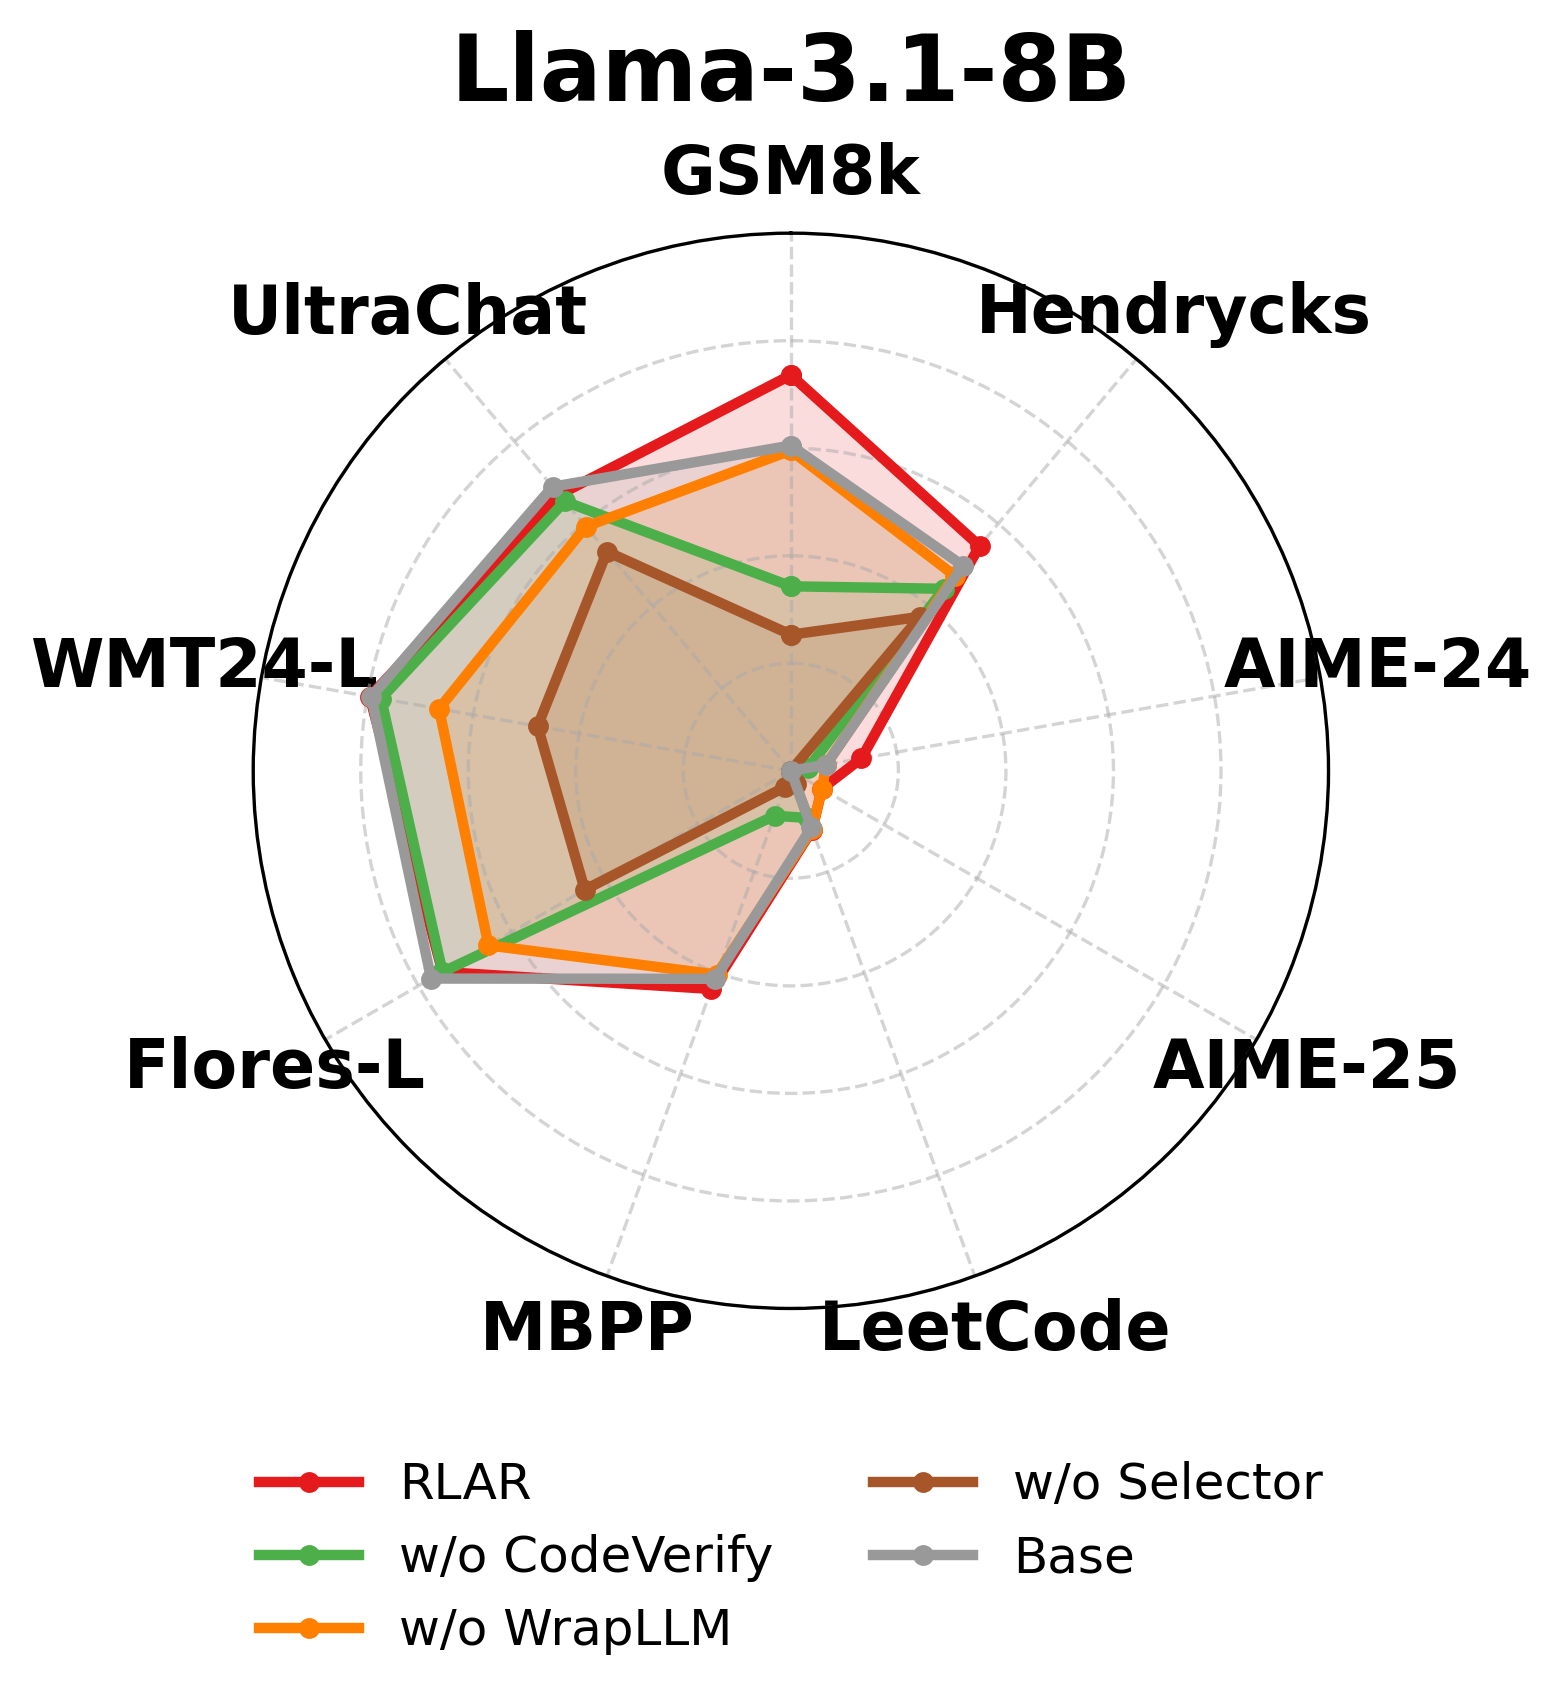
\includegraphics[width=\linewidth]{Figures/llama_ablation.png}
        \caption{Llama-3.1-8B}
        \label{fig:abl_llama}
    \end{subfigure}\hfill
    \begin{subfigure}{0.48\linewidth}
        \centering
        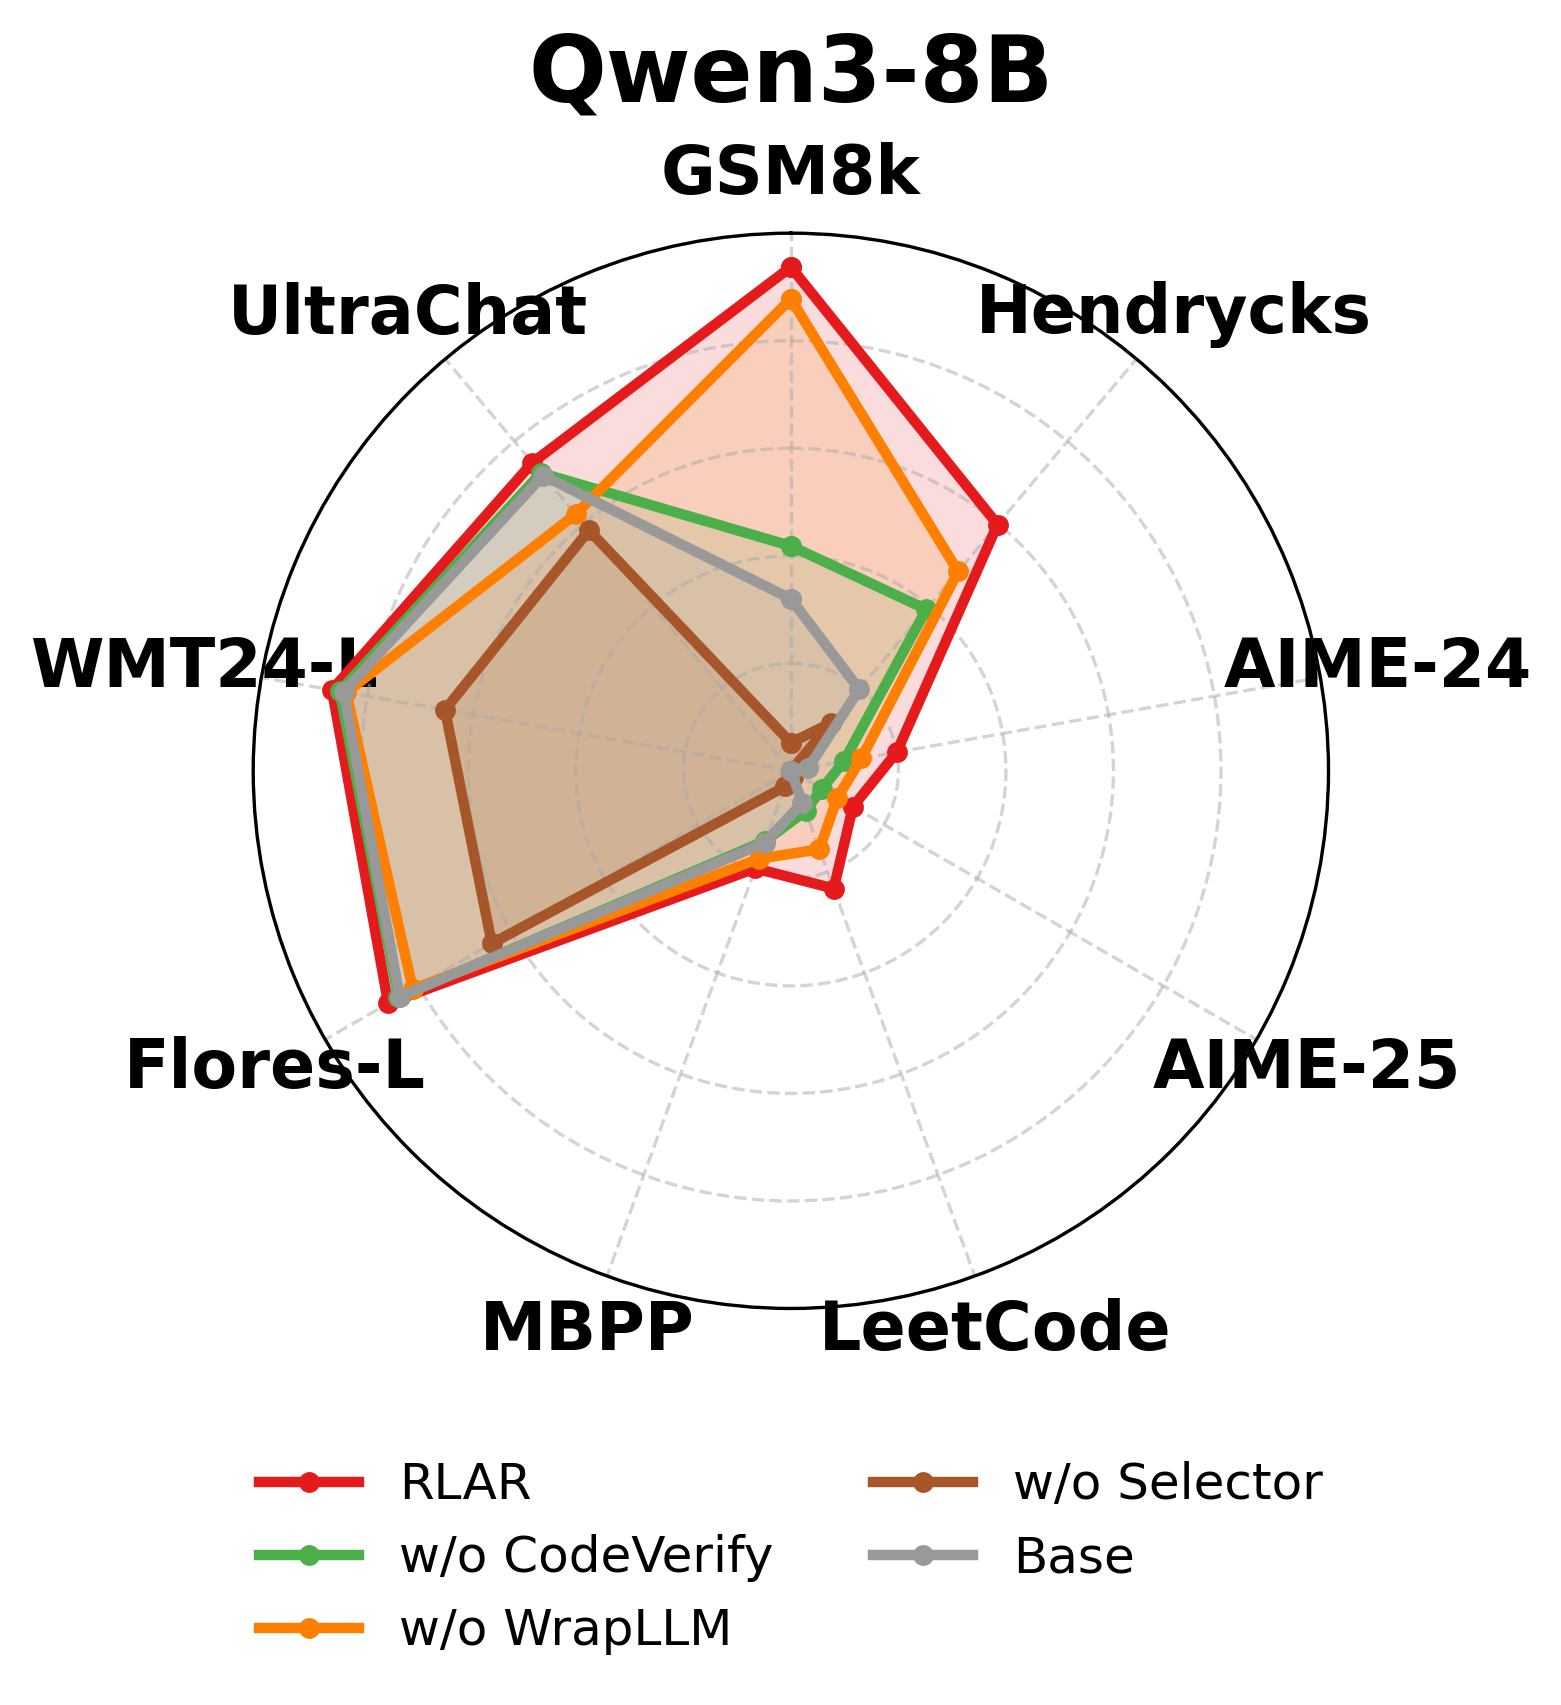
\includegraphics[width=\linewidth]{Figures/qwen_ablation.png}
        \caption{Qwen3-8B}
        \label{fig:abl_qwen}
    \end{subfigure}
    \caption{Ablation studies on Llama-3.1 and Qwen3.}
    \label{fig:ablation}
    \vspace{-4mm}
\end{wrapfigure}




\noindent\textbf{Hack with Verbosity.} \quad
Furthermore, we observe a persistent verbosity bias in LLM-based reward baselines. For example, models trained with GPT-5-Judge consistently produce outputs \(30\%\) \textbf{longer} than those partly learned from rule-based rewards (Human/RLAR). This confirms that verbosity bias is inherently latent in reward LLMs and can be triggered during RL.
Due to its rewarding versatility and the abundant included verifiable rewards, \method{} does not introduce a significant long-tail generation problem.




